\documentclass[10pt]{article}

% Lines beginning with the percent sign are comments
% This file has been commented to help you understand more about LaTeX

% DO NOT EDIT THE LINES BETWEEN THE TWO LONG HORIZONTAL LINES

%---------------------------------------------------------------------------------------------------------

% Packages add extra functionality.
\usepackage{times,graphicx,epstopdf,fancyhdr,amsfonts,amsthm,amsmath,algorithm,algorithmic,xspace,hyperref}
\usepackage[left=1in,top=1in,right=1in,bottom=1in]{geometry}
\usepackage{sect sty}	%For centering section headings
\usepackage{enumerate}	%Allows more labeling options for enumerate environments 
\usepackage{epsfig}
\usepackage[space]{grffile}
\usepackage{booktabs}
\usepackage{forest}
\usepackage{enumitem}   
\usepackage{fancyvrb}
\usepackage{todonotes}

% This will set LaTeX to look for figures in the same directory as the .tex file
\graphicspath{.} % The dot means current directory.

\pagestyle{fancy}

\lhead{Final Project}
\rhead{\today}
\lfoot{CSCI 334: Principles of Programming Languages}
\cfoot{\thepage}
\rfoot{Spring 2024}

% Some commands for changing header and footer format
\renewcommand{\headrulewidth}{0.4pt}
\renewcommand{\headwidth}{\textwidth}
\renewcommand{\footrulewidth}{0.4pt}



% These let you use common environments
\newtheorem{claim}{Claim}
\newtheorem{definition}{Definition}
\newtheorem{theorem}{Theorem}
\newtheorem{lemma}{Lemma}
\newtheorem{observation}{Observation}
\newtheorem{question}{Question}

\setlength{\parindent}{0cm}

%---------------------------------------------------------------------------------------------------------

% DON'T CHANGE ANYTHING ABOVE HERE

% Edit below as instructed

\title{Dot Language Specification} % Replace SnappyLanguageName with your project's name

\author{David Vieten} % Replace these with real partner names.

\begin{document}
  
\maketitle

\subsection*{Introduction}
{Fortunately, I have had the privilege of being around the sport of
hockey for the majority of my lifetime. Over the years, it has become clear to me that 
the current method of drawing face-off plays is outdated and inefficient. A face-off takes place on a face-off dot
 at the start of a period or following a whistle. The ref drops the puck on the face-off dot and two center-men battle 
 for possesion. Face-offs play an important role in hockey, as they serve as opportunity to gain possession and run a set 
 play. As a result, coaches draw up routes for each of the 5 guys on the ice, dictating the duty of each player off of a 
 face-off.  Often, teams have multiple versions of these set routes called "face-off plays." These
face-off plays may change on any given week depending on who the opponent is and what their weaknesses
are. As a result, the players are responsible for memorizing their routes. Currently, coaches either draw
up the faceoff plays on a white board and hope the players can remember it, or they draw them up on paper
and distribute photocopies for the players to study.\\


The programming language Dot solves this problem. Dot allows coaches to create face-off plays in an SVG, which can then
be sent out to the players. These face-off plays can be drawn on any offensive zone or defensive zone face-off dot. 
This language saves coaches a headache by providing a way to easily distribute
face-off plays without wasting paper and ink to do so. Coaches will also be able to save face-off plays,
allowing them to keep track of what plays they have used against who in the past. This ability to save face-off
plays will allow coaches to save scouting reports, increasing prepardness for the team. In a typical game week, coaches 
will watch video on the opposing team to get an idea of what they will be faced with come game time. While watching video, 
coaches can create and save the opposing team's faceoff plays to determine the best counter plays. Dot will save coaches 
time and allow players to study their routes in an efficient manner.
}

\subsection*{Design Principles}
{Several design principles guide Dot's development to address the problem of creating and
distributing faceoff plays. With the goal of accessibility and usability, Dot produces an
SVG allowing coaches to easily distribute visual representations of plays. Efficiency is another principle that Dot seeks to achieve.
The ability to save and organize face-off plays supports this by allowing coaches to easily create libraries
of strategies/pre-scouts over time. Extensibility is also a fundamental design principle in the
development of the language. Dot allows for the creation of custom plays designed for specific opponents, providing
an advantage in the hockey world. With the current infrastructure, Dot provides a way to create an extensive number of plays.
 Furthermore, Dot's support for saving and analyzing opponent's face-off plays
contributes to its strategic use as a tool for planning and adapting. Moreover, Dot is built with accessibility,
efficiency, and extensability in mind.
}

\pagebreak
\subsection*{Examples}

\begin{enumerate}
  \item
  dotnet run Boston.dot

  \begin{verbatim}
  <svg width="400" height="400" xmlns="http://www.w3.org/2000/svg">
  <image href="Rink.png" height="400" width="400" />
  <circle cx="239" cy="250" r="5" fill="black" />
  <circle cx="200" cy="300" r="5" fill="black" />
  <line x1="239" y1="250" x2="200" y2="300" style="stroke:black;stroke-width:3" />
  <circle cx="353" cy="250" r="5" fill="black" />
  <circle cx="363" cy="350" r="5" fill="black" />
  <line x1="353" y1="250" x2="363" y2="350" style="stroke:black;stroke-width:3" />
  <circle cx="296" cy="250" r="5" fill="black" />
  <circle cx="200" cy="270" r="5" fill="black" />
  <line x1="296" y1="250" x2="200" y2="270" style="stroke:black;stroke-width:3" />
  <circle cx="239" cy="160" r="5" fill="black" />
  <circle cx="139" cy="160" r="5" fill="black" />
  <line x1="239" y1="160" x2="139" y2="160" style="stroke:black;stroke-width:3" />
  <circle cx="353" cy="160" r="5" fill="black" />
  <circle cx="376" cy="220" r="5" fill="black" />
  <line x1="353" y1="160" x2="376" y2="220" style="stroke:black;stroke-width:3" />
  </svg>
  \end{verbatim}

\item
  dotnet run Ephs.dot 
  \begin{verbatim}
  <svg width="400" height="400" xmlns="http://www.w3.org/2000/svg">
  <image href="Rink.png" height="400" width="400" />
  <circle cx="249" cy="310" r="5" fill="black" />
  <circle cx="356" cy="350" r="5" fill="black" />
  <line x1="249" y1="310" x2="356" y2="350" style="stroke:black;stroke-width:3" />
  <circle cx="353" cy="280" r="5" fill="black" />
  <circle cx="183" cy="310" r="5" fill="black" />
  <line x1="353" y1="280" x2="183" y2="310" style="stroke:black;stroke-width:3" />
  <circle cx="296" cy="280" r="5" fill="black" />
  <circle cx="200" cy="270" r="5" fill="black" />
  <line x1="296" y1="280" x2="200" y2="270" style="stroke:black;stroke-width:3" />
  <circle cx="239" cy="280" r="5" fill="black" />
  <circle cx="239" cy="280" r="5" fill="black" />
  <line x1="239" y1="280" x2="239" y2="280" style="stroke:black;stroke-width:3" />
  <circle cx="353" cy="310" r="5" fill="black" />
  <circle cx="383" cy="230" r="5" fill="black" />
  <line x1="353" y1="310" x2="383" y2="230" style="stroke:black;stroke-width:3" />
  </svg>
  \end{verbatim}

  \pagebreak
\item
  dotnet run Maverick.dot MavSVG\\
  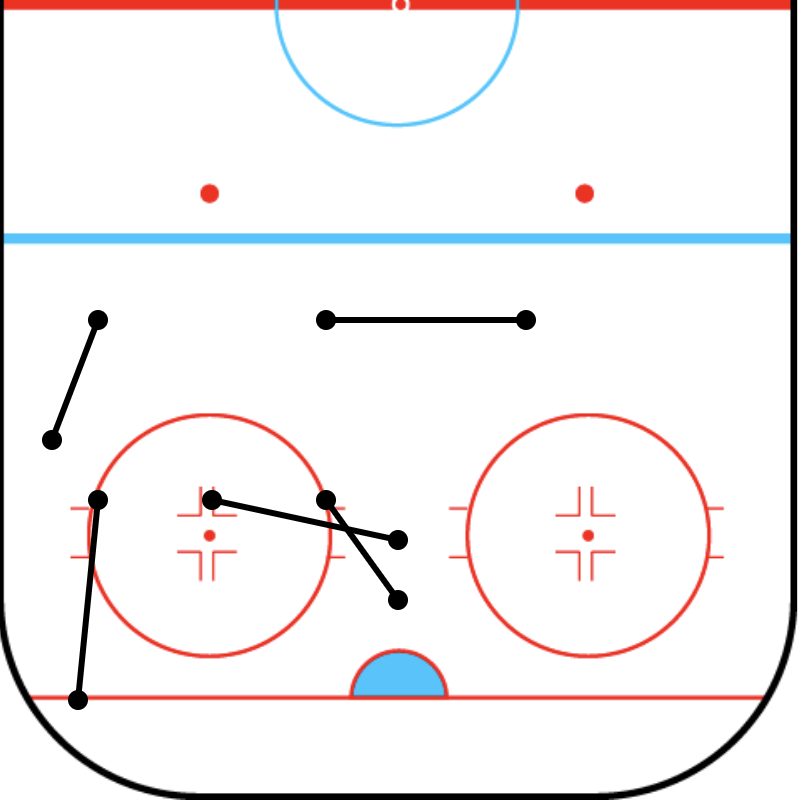
\includegraphics[width=10cm]{images/Mav1}
\end{enumerate}


\subsection*{Language Concepts}

To write programs in this language, users need to have a grasp on the concepts of primitives and combining forms as 
well as knowledge of the sport of hockey. The primitives help define areas on the hockey rink through the use of side
 and zone indicators to specify the context of the location.  End routes represent endpoints 
 that players will move to from their original position once the puck drops. Combining forms involve creating these routes 
 by pairing start and end points. These routes can be organized into a board, which is a list of routes. A sequence of 
 strategic moves can then be represented off a faceoff. By understanding these core concepts, users can effectively design 
 player movements that will produce an advantage on game day.\\

 Aside from that, the techincal aspect of using the project is simple. Users will create a .dot file
 containing 1 or more routes. For more information please refer to the formal syntax, but a typical route will include a 
 starting postion, an ending position, and should specify the side and zone on the ice. Once this file is saved, the user can create their svg file on the command line. Users will type
 \textbf{dotnet run $<$someDotFile$>$ w}hich will return a string representing an svg. Using this string, users will be able to create their svg.
 To further simply this, I have created an option to create the SVG itself from the command line rather than return an svg string.
 Users should follow the same directions as before, typing \textbf{dotnet run $<$someDotFile$>$}, but now followed by the desired name of the svg 
 file that will be produced. Running \textbf{dotnet run $<$someDotFile$>$ $<$newSvgFile$>$} take someDotFile.dot as input and produce and save an 
 SVG named newSvgFile.svg. The users computer will then open newSvgFile in their default SVG viewer.


 \pagebreak
\subsection*{Formal Syntax}
\begin{verbatim}
        <expr> ::= <route>+
        <route>::= <routedef><dotplace>
    <routedef> ::= <startroute><endroute>
    <dotplace> ::= <side><zone>
    <endroute> ::= net
                | walkline
                | halfwall
                | corner
                | hold
                | slot
                | backdoor   
 <startroute> ::= lefthash
                |  righthash
                |  dot
                |  rightpoint
                |  leftpoint
                |  stackinside
                |  stackoutside   
        <zone> ::= offense
                |  defense
        <side> ::= right
                |  left
   \end{verbatim}
\pagebreak
   \subsection*{Semantics}
   \begin{table}[htbp]
     \centering
     \caption{Semantics of Language}
     \begin{tabular}{|p{2cm}|p{4cm}|p{6cm}|}
       \hline
       \textbf{Syntax} & \textbf{Abstract Syntax} & \textbf{Meaning} \\
       \hline
       \textless side\textgreater{}& Side of string & side is primitive. Represents the sides of the ice: "right" or "left". \\
       \hline
       \textless zone\textgreater{}& Zone of string & zone is primitive. Represents the zones of the ice where players will line up.: "offense" or "defense". \\
       \hline
       \textless route\textgreater{} & Route of RouteDef * DotPlace & route is a combing form. Represents a route of a player on the ice, defined by a route definition and a dot placement. Route is a record of RouteDef and DotPlace. \\
       \hline
       \textless routedef\textgreater{} & RouteDef of StartRoute * EndRoute & routedef is a combining form. Represents the definition of a route, consisting of a start point and an end point. Dictates the coordinates of startroute and endroute. RouteDef is a tuple of StartRoute and EndRoute. \\
       \hline
       \textless dotplace\textgreater{} & DotPlace of Side * Zone & dotplace is combining form. Represents the placement of a dot along a route, defined by side and zone. DotPlace is a tuple of Side * Zone\\
       \hline
       \textless startroute\textgreater{} & StartRoute of string & startroute is a primitive. Represents the possible starting points or areas of a route. Eval turns these into coordinates. \\
       \hline
       \textless endroute\textgreater{} & EndRoute of string & endroute is a primitive. Represents the possible ending points of a route. Eval turns these into coordinates.\\
       \hline
     \end{tabular}
   \end{table}

  \pagebreak
\subsection*{Remaining Work}
{Right now, Dot is capable of producing routes for a single team, either on the offensive
or defensive side of the dot. The next step to further improve this langauge is to 
incorporate the ability to show players either skating with or passing the puck. This requires
drawing dotted and squiggly lines as opposed to stright lines. By doing this, players would know
their routes of the face-off, as well as the where the puck will be. Given our set time period,
I am unable to implement this feature. With some more experience in SVG, I think I could add 
this feature, and it would greatly enhance the abilities of Dot. \\

Along with this feature, creating the ability to draw routes on neutral zone dots would enhance the user
exerience. There are a few ways this could be implemented, but I think the most straight forward would be to add
a match case in the evaluation step that would dictate which .png is imported. This would change the grammar of the language,
asking users to specify if a face-off should take place in the nuetral zone or not. Similar to the first feature, I believe this
could be implemented with some more time allowed.}

% DO NOT DELETE ANYTHING BELOW THIS LINE
\end{document}